\documentclass[../doc.tex]{subfiles}

\begin{document}

    Le menu d'accueil est la première chose que le joueur voit en lançant le jeu.
    Celui-ci est actuellement entièrement implémenté et fonctionnel. Cependant il continuera 
    d'évoluer au fil du projet et de ses besoins.

    \paragraph{Thème général}
    Le thème du menu principal doit être représentatif du jeu. Il doit donc bien entendu 
    afficher la couleur dès le lancement: ceci est un jeu de pirates.
    Le fond, les couleurs, la musique... Y est également présent le logo du 
    groupe ainsi que celui du jeu.
    
    \paragraph{Fonctionnalités}
    Plusieurs options sont disponibles. Le joueur peut tout d'abord se connecter 
    au serveur Photon. Il accède ainsi à un menu lui permettant de rejoindre une 
    salle. Il peut également y modifier son pseudo, qui sera affiché aux autres 
    joueurs. Seule la fonction "Quick Play" a été implémentée (cf. multijoueur) mais 
    l'objectif à long terme est d'ajouter une liste ainsi qu'un menu de création de 
    salles. Cette partie du menu principal a été réalisée par Julien.
    
    Il est également possible de modifier les paramètres de jeu comme la 
    résolution, le mode plein écran, le volume, ou encore remapper les touches de 
    contrôles. Ces changements sont sauvegardés (cf. système de sauvegardes).
    
    Un menu de personnalisation de personnage a également été implémenté 
    (cf. système de progression). On peut y modifier certaines caractéristiques, 
    comme la couleur des vêtements ou de la peau. Un aperçu du modèle est disponible 
    (et peut pivoter grâce à la souris). Les paramètres, ainsi que ce menu, ont été 
    réalisés par Harrys.
    
    Enfin, on retrouve (évidemment) un bouton quitter pour fermer l'application.
    
    \begin{figure}[hbt!]
                \centering
                \captionsetup{justification=centering}
                \begin{subfigure}[b]{0.3\textwidth}
                    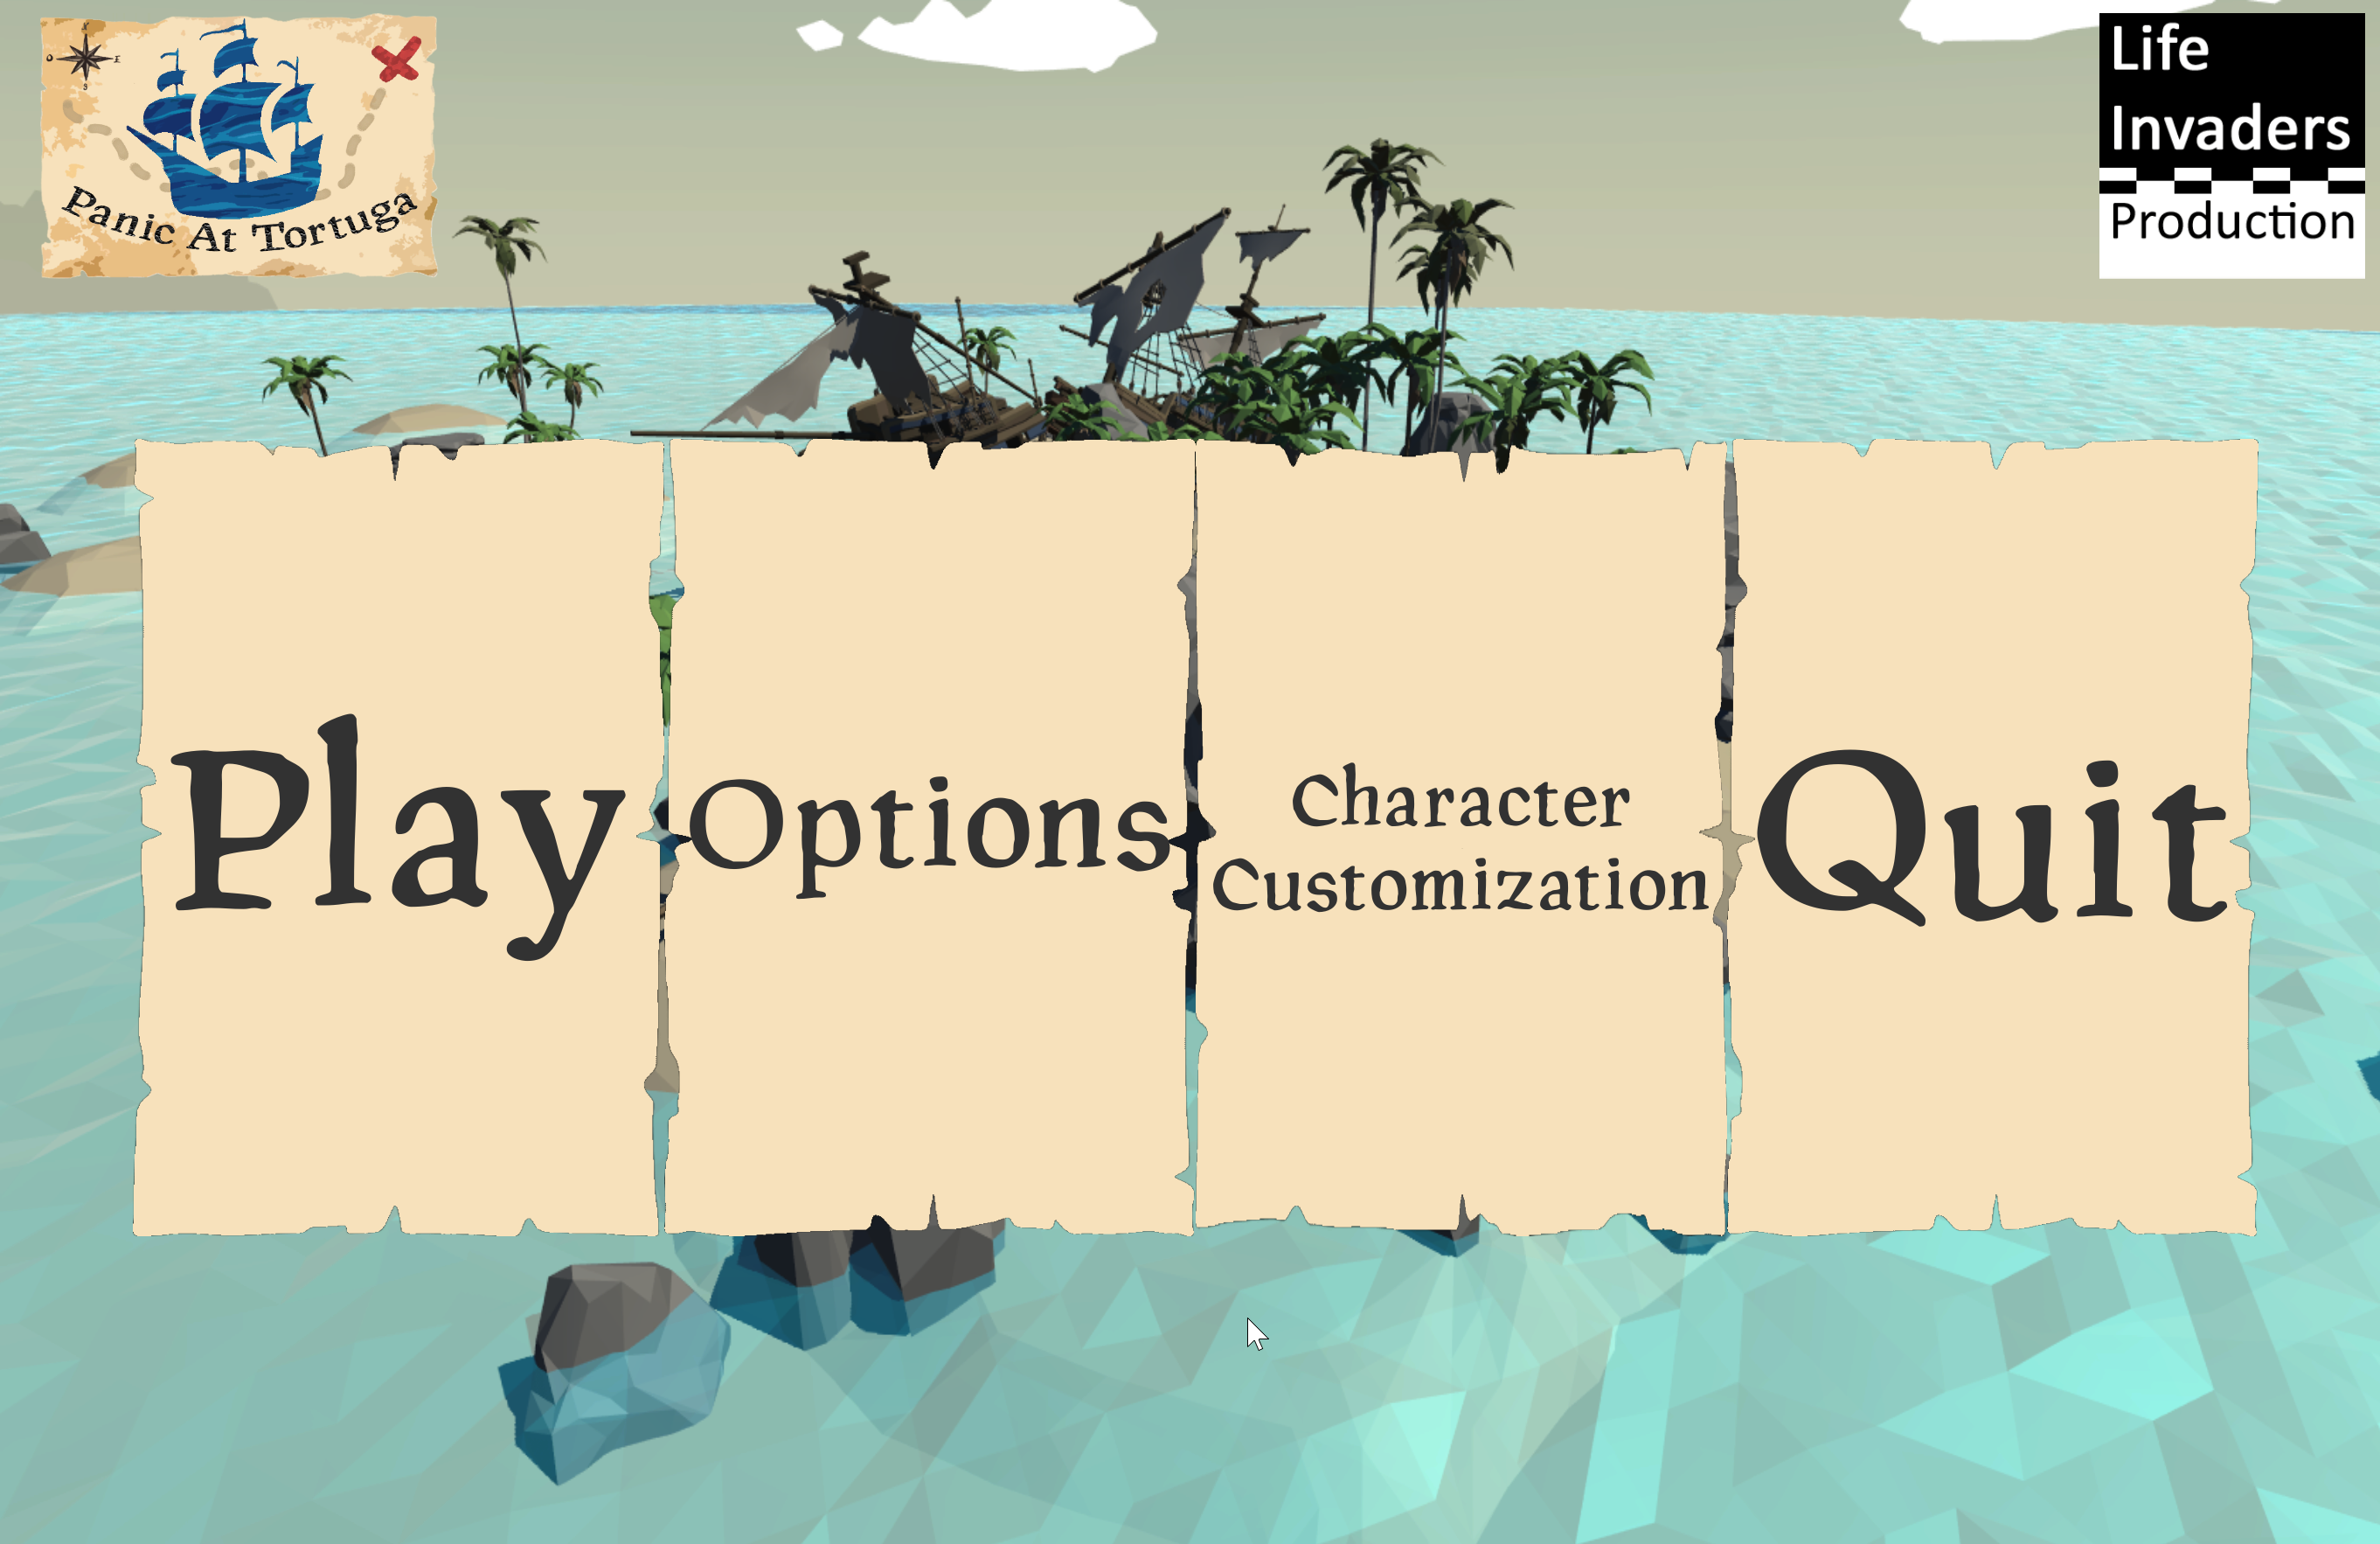
\includegraphics[scale=0.1]{mainmenu.png} 
                    \caption{Menu principal}
                \end{subfigure}
                \hspace{150pt}
                \begin{subfigure}[b]{0.3\textwidth}
                    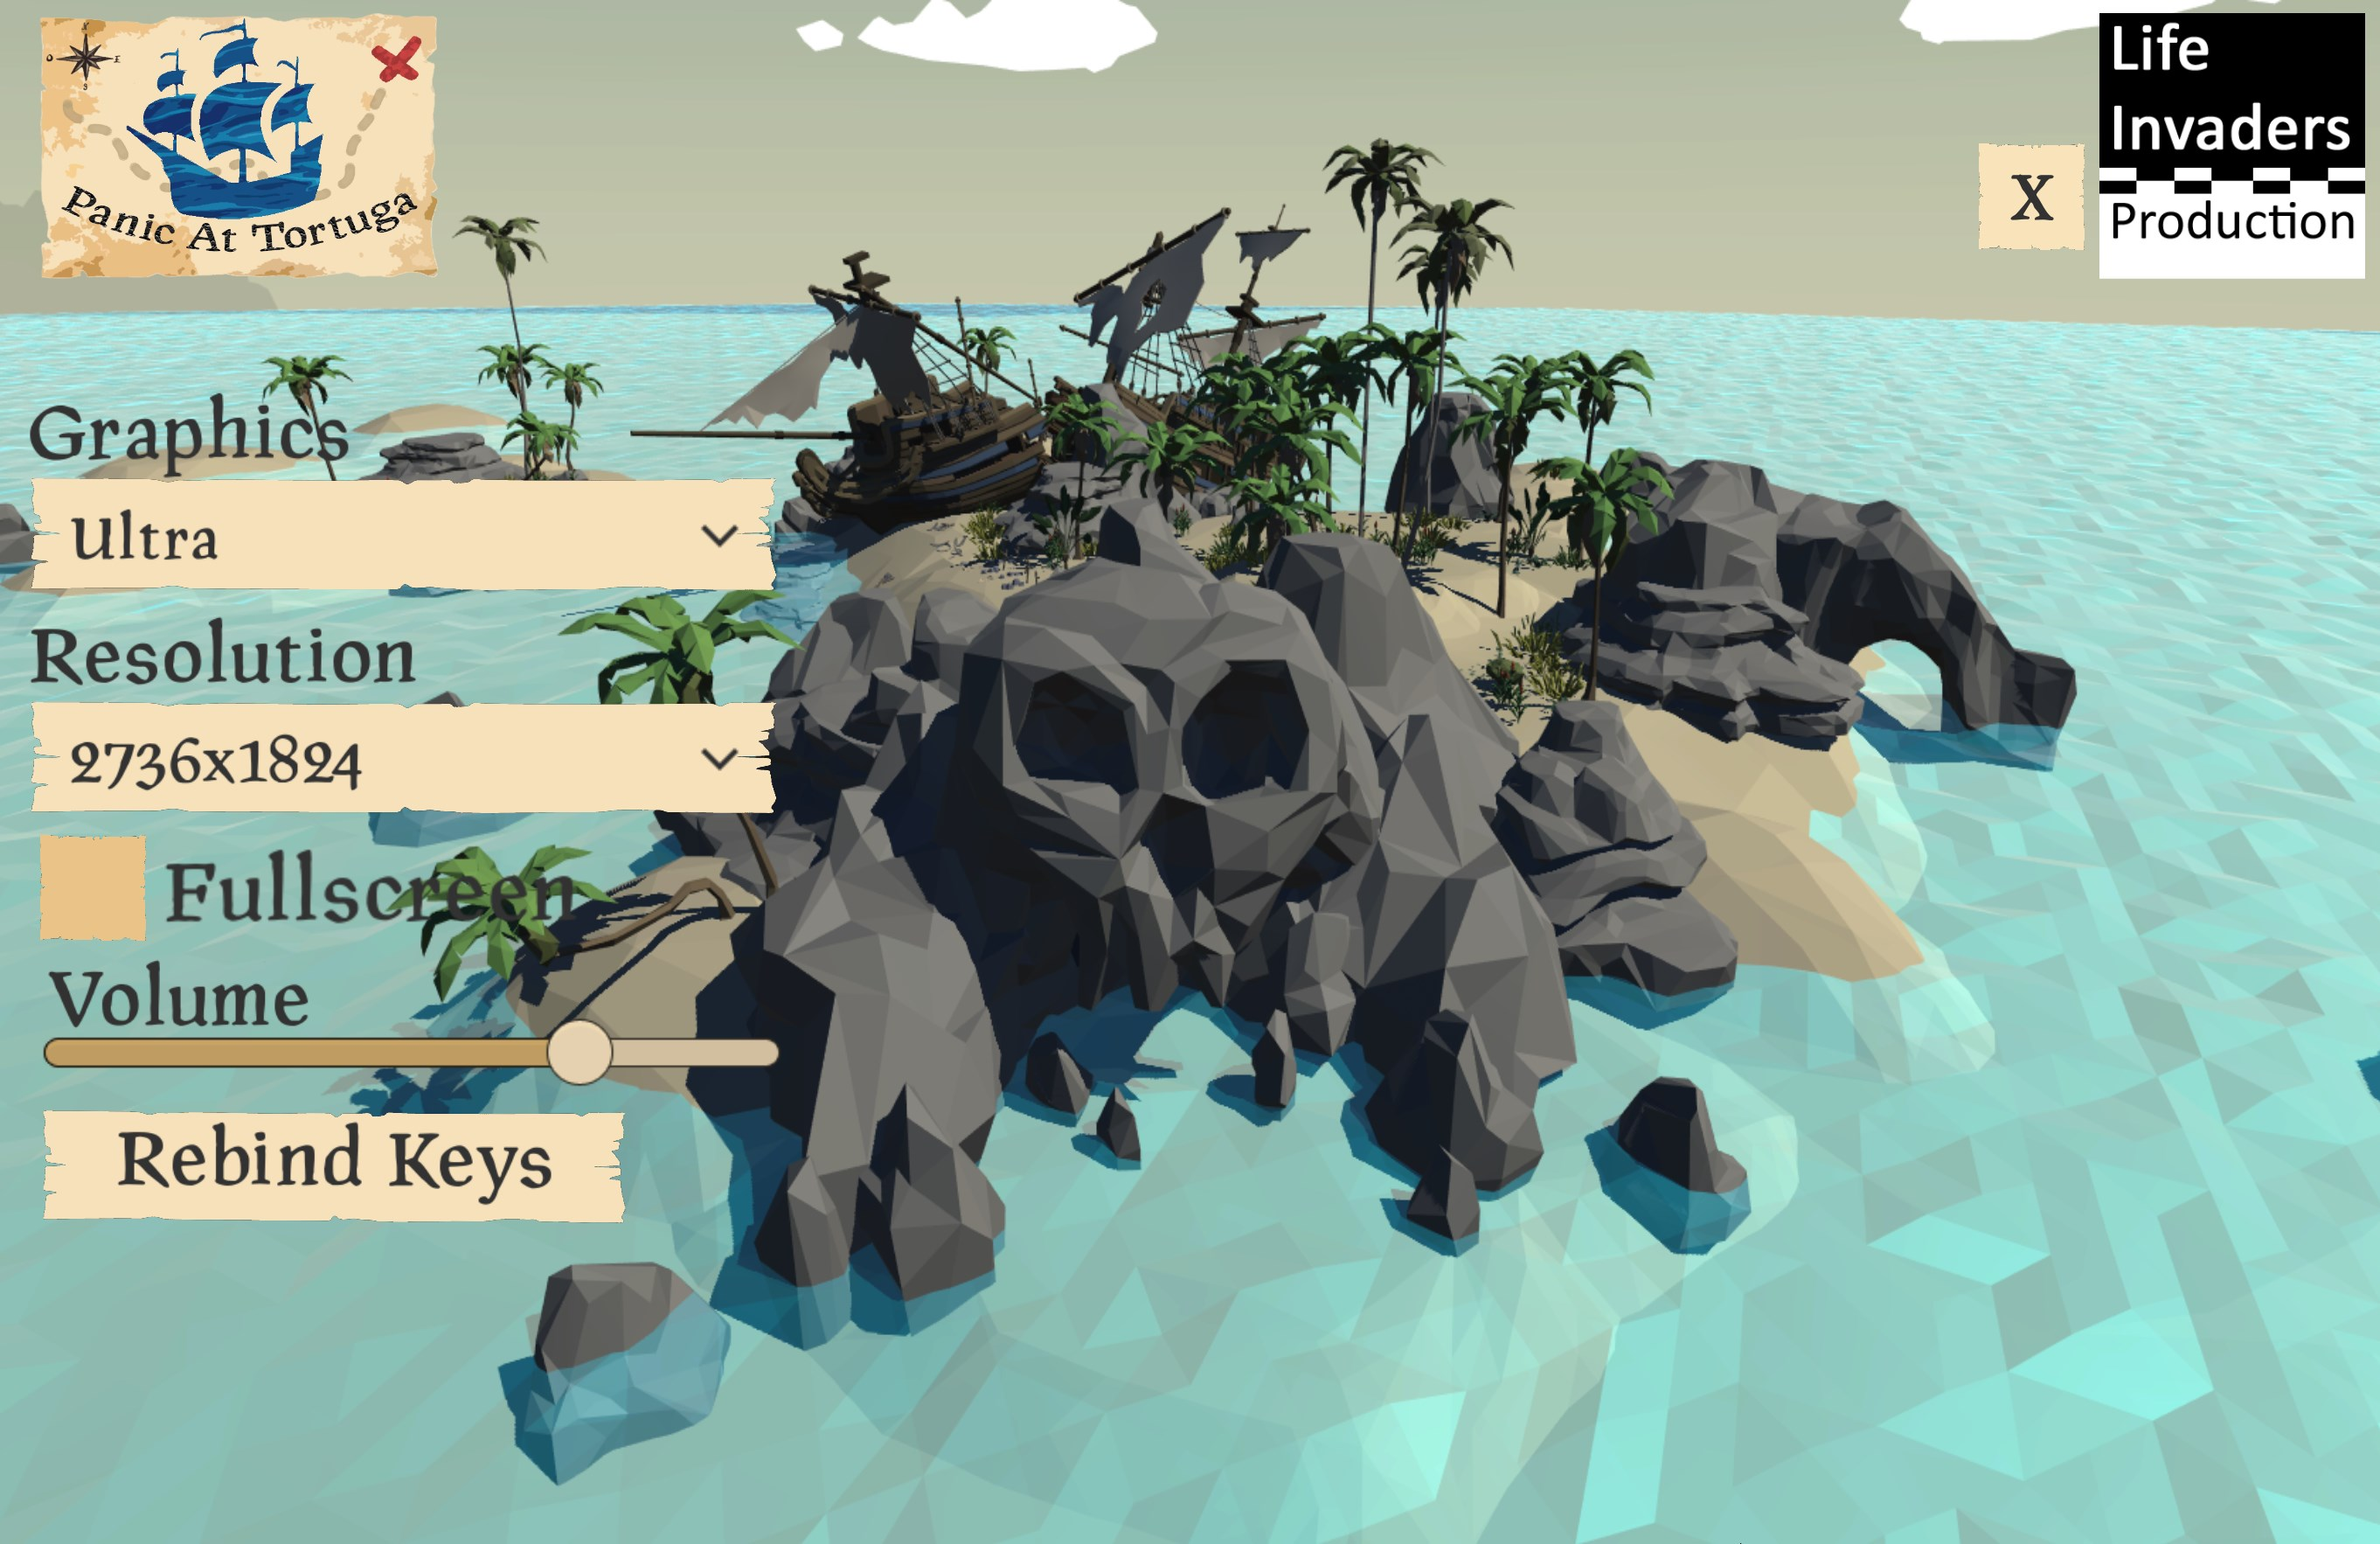
\includegraphics[scale=0.1]{settingsmenu.jpg} 
                    \caption{Paramètres}
                \end{subfigure}
                \begin{subfigure}[b]{0.3\textwidth}
                    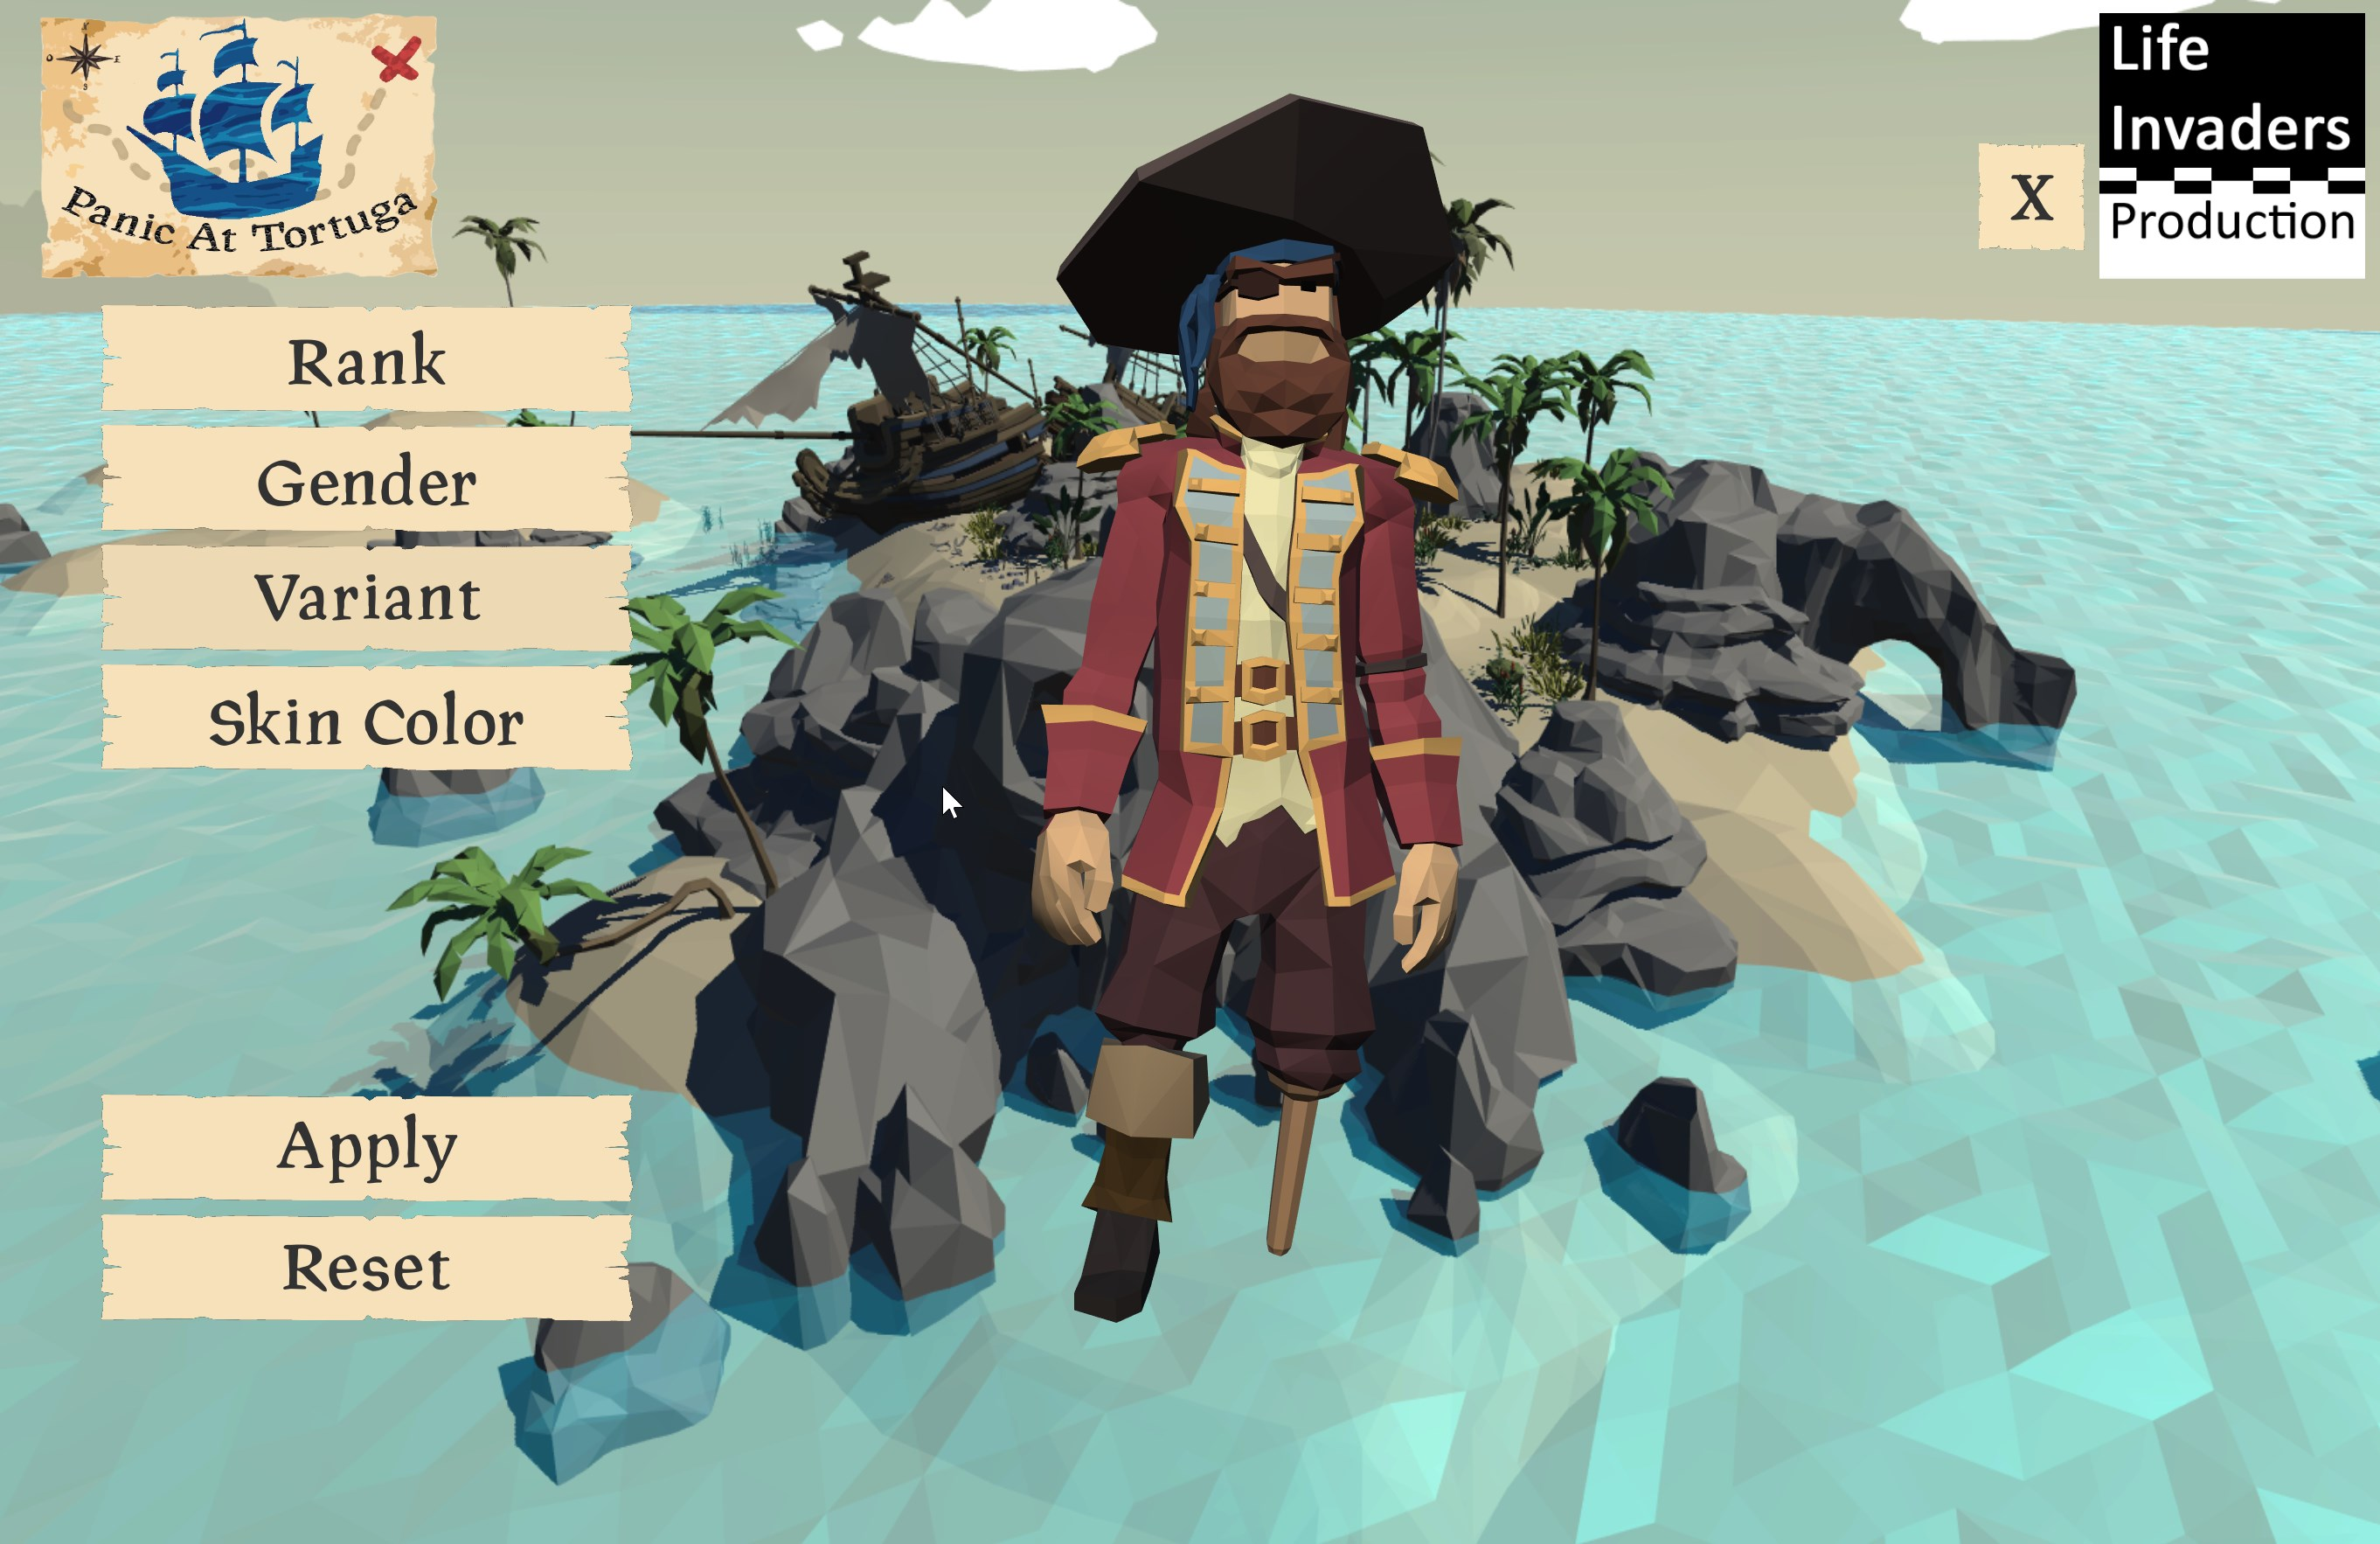
\includegraphics[scale=0.1]{charcustom.jpg} 
                    \caption{Apparence}
                \end{subfigure}
                \begin{subfigure}[b]{0.3\textwidth}
                    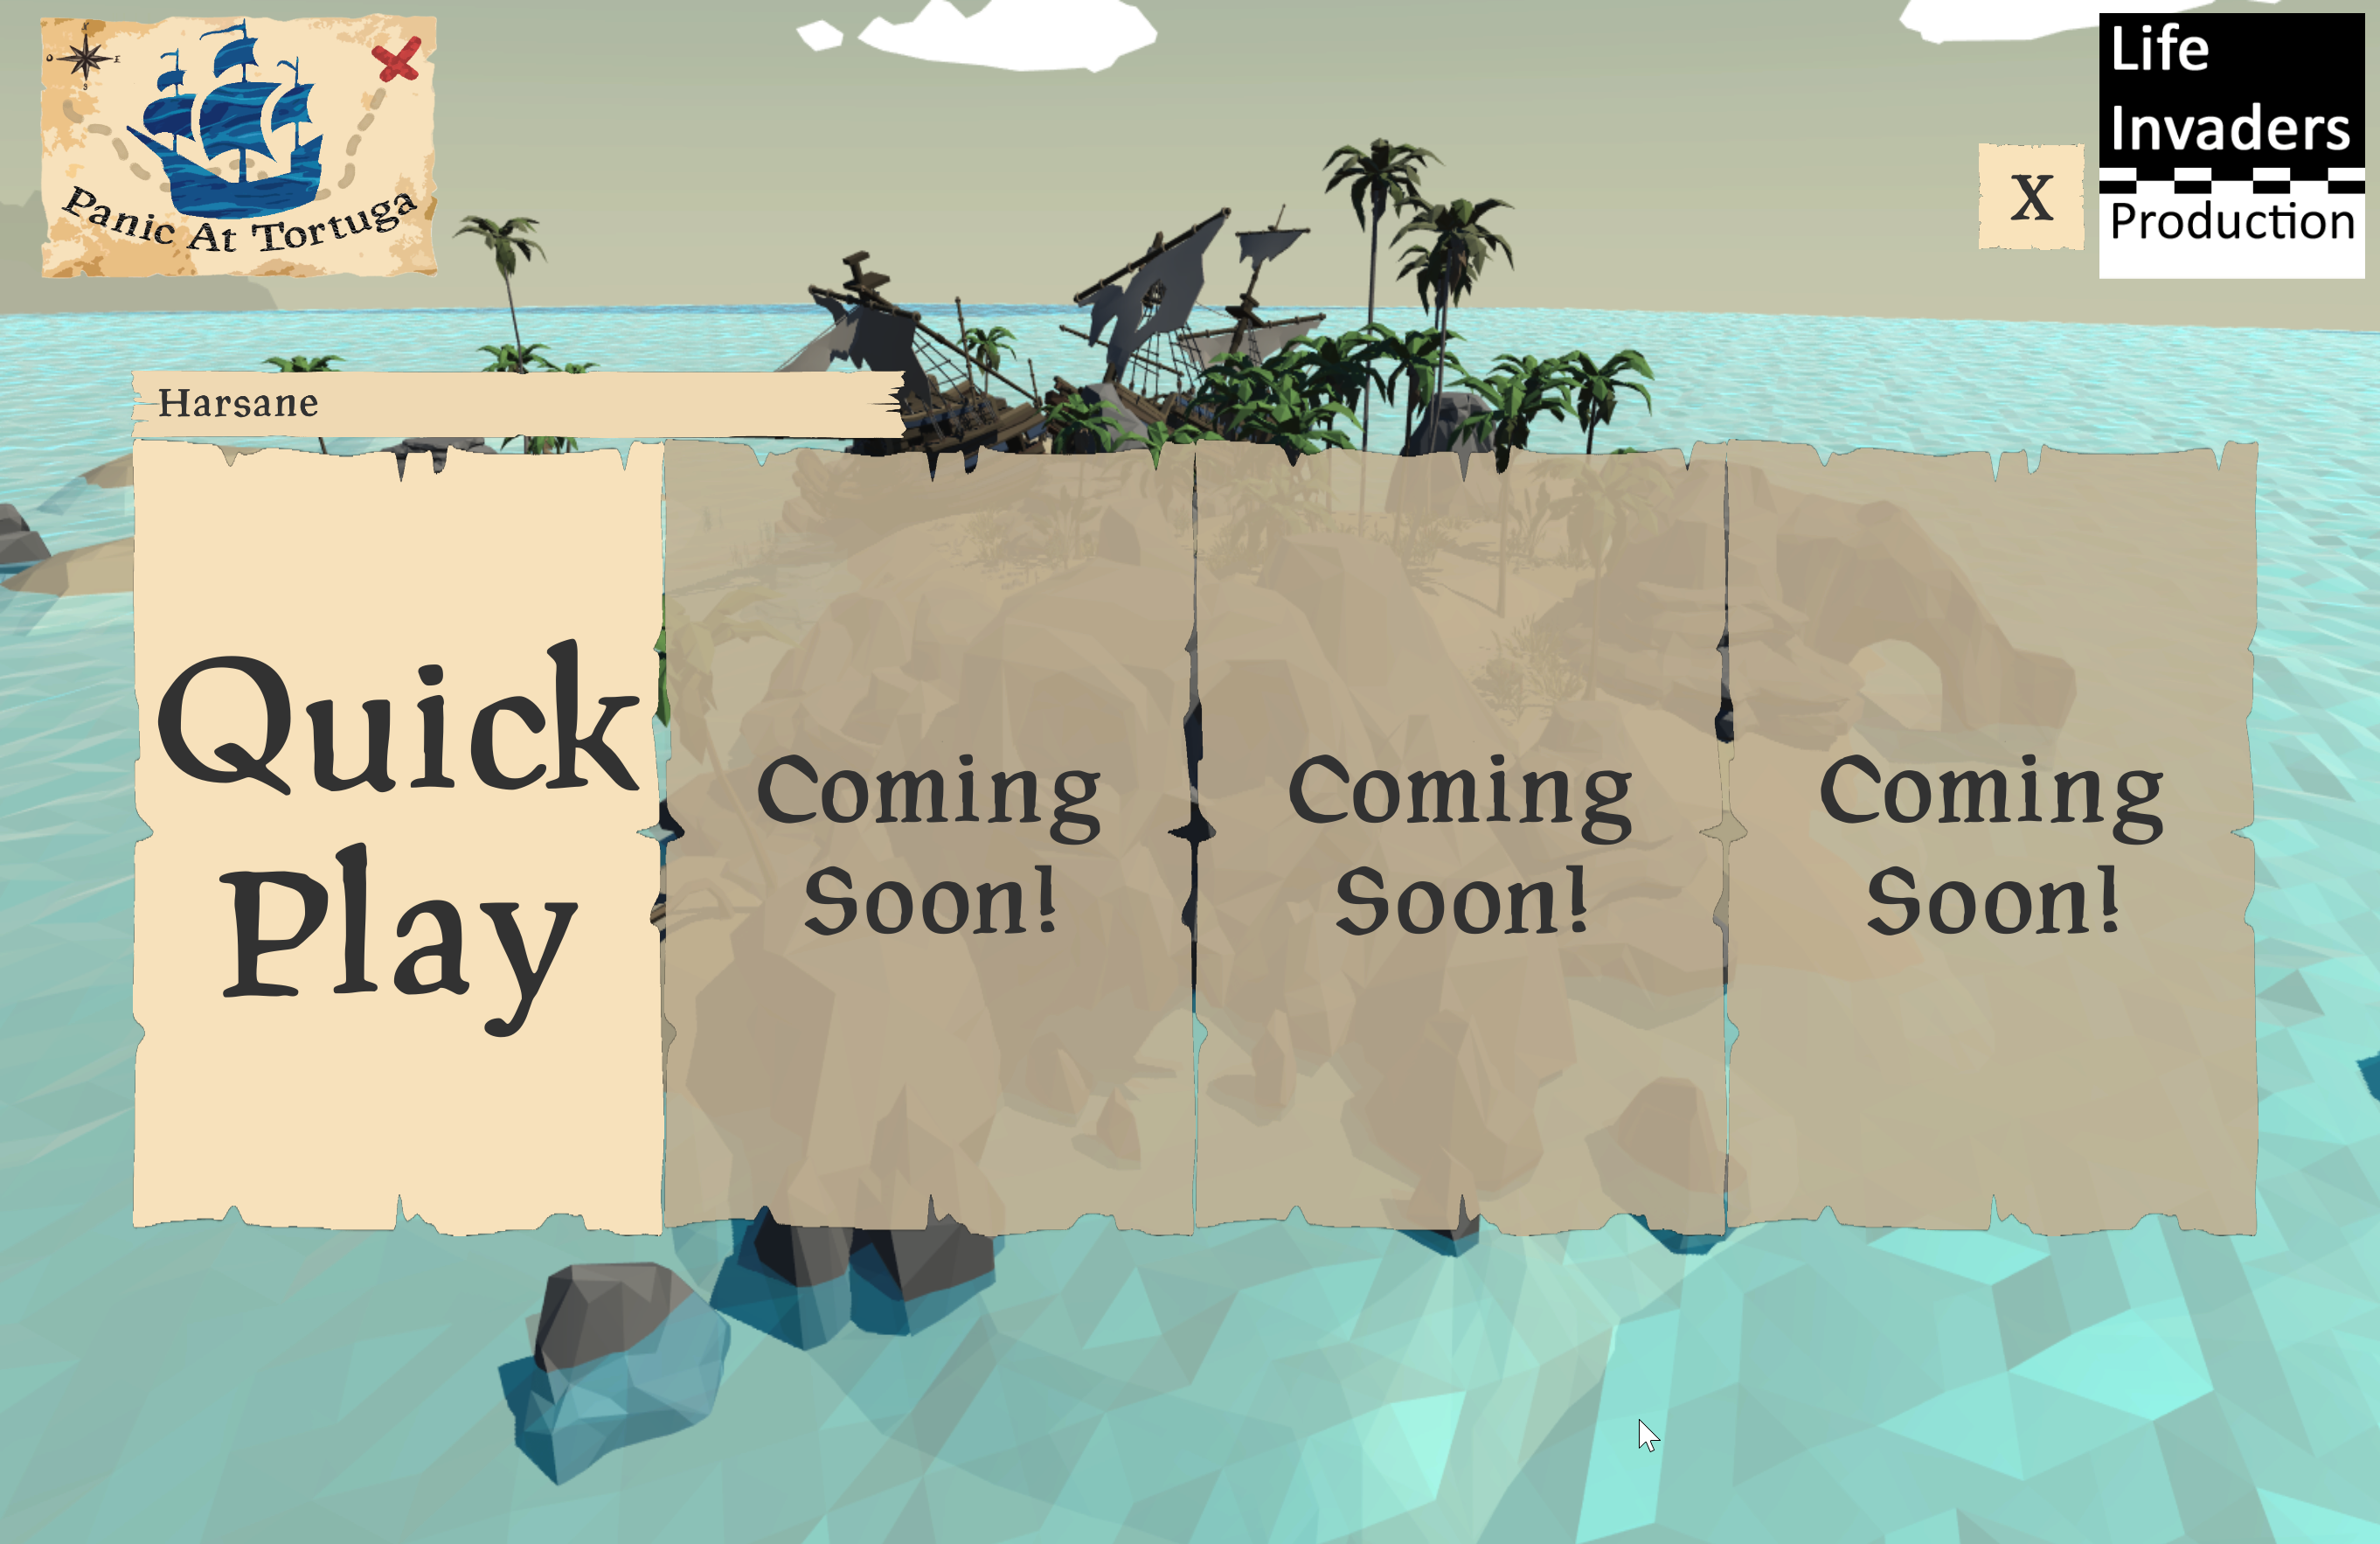
\includegraphics[scale=0.1]{photonmenu.png} 
                    \caption{Menu multijoueur}
                \end{subfigure}
                \caption{Différents affichages du menu d'accueil}
    \end{figure}

\end{document}
